% !TeX spellcheck = en_US
%!TeX spellcheck = el_EL-ModernGreek
\documentclass[12pt,a4paper]{article}
\usepackage[utf8]{inputenc}
\usepackage[T1]{fontenc}
\usepackage{amsmath}
\usepackage{amssymb}
\usepackage{graphicx}
\usepackage{fancyhdr}
\usepackage[left=1.50cm, right=1.50cm, top=1.50cm, bottom=1.50cm, includeheadfoot]{geometry}
\usepackage[greek]{babel}
\usepackage{fontspec}
\setmainfont{Verdana}
\usepackage[hidelinks]{hyperref}
\usepackage{subfigure}
\usepackage{dirtree}
\usepackage{float}
\usepackage{wrapfig}
\usepackage{color}
\usepackage[dvipsnames]{xcolor}
\usepackage{fontawesome}
\usepackage{pifont}
\usepackage{eso-pic}
\usepackage{fancyhdr}


\pagestyle{fancy}
\lhead{\textcolor{blue}{SoC Report} }
\rhead{\textcolor{blue}{Reed Solomon Decoder with UART} }
\setlength{\headheight}{15pt}


\title{\textbf{\textcolor{red}{\underline{Reed Solomon Decoder with UART}} } }
\author{Δημήτρης Τσαλαπάτας - Γιάννης Ρείνος}
\date{10 Ιουλίου 2023}

\begin{document}

\AddToShipoutPictureBG*{
	\put(10, 720){
		\includegraphics[width=4cm,height=4cm]{UTH.png}
	}
}

\AddToShipoutPictureBG*{
	\put(470, 720){
		\includegraphics[width=4cm,height=4cm]{ece.png}
	}
}

	\maketitle
	\tableofcontents
	\newpage
	\section{\textcolor{PineGreen}{General Description of Design} }
    Το design που επιλέξαμε να υλοποιήσουμε είναι ένας \verb|Reed Solomon Decoder| ο οποίος λαμβάνει δεδομένα μέσω ενός UART Receiver. Θεωρούμε ότι λαμβανουμε τα δεδομένα από έναν αντίστοιχο encoder ο οποίος τα στέλνει μέσω UART Transmitter. Τα δύο modules σύνδεονται μέσω μίας FSM που υλοποιήσαμε, η οποία συλλέγει μέσω του Receiver τα δεδομένα και κάθε φορά που ένα μήνυμα είναι έτοιμο το προωθεί στον Decoder για να γίνει η αποκωδικοποίηση. \\
    Παρατίθεται παρακάτω το top level Dataflow για το design
    
     \begin{figure} [htbp]
     	\centering{\includegraphics[width=\textwidth]{dataflow1.drawio.png} }
     	\caption{Top view Dataflow}
     	\label{Top view Dataflow}
     \end{figure}

    
	
	\section{\textcolor{PineGreen}{UART Receiver} }
    Αρχικά, χρησιμοποιείται στο design ένας \verb|UART| Receiver δικιάς μας υλοποίησης, ο οποίος λαμβάνει πακέτα των 8 bits σε όλες τις πιθανές ταχύτητες που υποστηρίζονται από το πρωτόκολλο του UART. O receiver λαμβάνει σειριακά 11 bits από τον Transmitter. Αρχικά ο transmitter στέλνει το \verb|start bit|, ώστε να ξεκινήσει η επικοινωνία, στην συνέχεια ακολουθούν τα 8 bits δεδομένα, ένα parity bit και τέλος ένα stop bit όπου σηματοδοτεί την λήξη της επικοινωνίας. Μέσω της FSM ο receiver δειγματολειπτεί στην μέση του κάθε bit που στέλνει ο Transmitter και εφόσον λάβει και τα 8 bits ελέγχει το parity του πακέτου και εάν είναι ίδιο με αυτό που έλαβε σημαίνει ότι τα δεδομένα στάλθηκαν σωστά. 'Οταν ληφθεί το stop bit τελειώνει η αποστολή του συγκεκριμένου πακέτου. Τέλος, έχουν ληφθεί τα δεδομένα, τα στέλνει παράλληλα σαν output μαζί με ένα σήμα \verb|Rx_VALID| για να δηλώσει ότι τα δεδομένα είναι έγκυρα.
    
     \begin{figure} [H]
     	\centering{\includegraphics[width=0.9\textwidth]{uart_timing.png} }
     	\caption{UART Communication example}
     	\label{UART Communication example}
     \end{figure}

     
	\subsection{\textcolor{PineGreen}{UART dataflow}}
    Παρακάτω φαίνεται το dataflow για το UART στο οποίο περιέχεται το module του baud controller, λειτουργία του οποίου είναι να παρέχει το σήμα για δειγματοληψία στον Receiver ανάλογα με την εκάστοτε ταχύτητα. Επίσης, υπάρχει μία FSM η οποία ελέγχει όλη την λειτουργία του κυκλώματος με την χρήση ενός counter, και τέλος χρησιμοποιείται και ένα SIPO (serial to pararel shifter) για να μετατρέπονται τα δεδομένα από σειριακά σε παράλληλα.
    
     \begin{figure} [H]
     	\centering{\includegraphics[width=0.8\textwidth]{Dataflow part C.jpg} }
     	\caption{UART dataflow}
     	\label{UART Dataflow}
     \end{figure}

    \section{\textcolor{PineGreen}{Reed Solomon Decoder}}
    Ο Reed-Solomon είναι ένας αλγόριθμος κωδικοποίησης που χρησιμοποιείται για τη διόρθωση σφαλμάτων στη μετάδοση και αποθήκευση δεδομένων. Ο κώδικας υλοποιείται με τη δημιουργία ενός συνόλου πολυωνύμων που χρησιμοποιούνται για την κωδικοποίηση των δεδομένων. Περιλαμβάνει κάποια parity bits, τα οποία του επιτρέπουν να ανιχνεύει και να διορθώνει σφάλματα με τη χρήση μαθηματικών αλγορίθμων.\\
    Στο design μας, χρησιμοποιούμε τον Reed Solomon Decoder, ο οποίος λαμβάνει ένα \verb|codeword| (κωδικοποιημένο από έναν encoder) μήκους 204 bytes και αφού τα αποκωδικοποιήση βγάζει output ένα \verb|codeword| μήκους 188 bytes.
    \begin{figure} [H]
     	\centering{\includegraphics[width=0.8\textwidth]{reed flow chart.png} }
     	\caption{Reed Solomon Decoder Flowchart}
     	\label{Reed Solomon Decoder Flowchart}
     \end{figure}
    
    \subsection{\textcolor{PineGreen}{Steps of Operation}}
    
    Για κάθε εισερχόμενο codeword, υπολογίζονται τα syndromes και το εισερχόμενo codeword αποθηκεύεται στα input pipelining memories.
    \begin{itemize}
        \item Τα syndromes θα χρησιμοποιηθούν για να πάρουμε το πολυώνυμο εντοπισμού σφάλματος (Lambda) χρησιμοποιώντας τον αλγόριθμο Berlekamp-Massey. Οι συντελεστές θα προέρχονται από το L1 έως το L8 που θα αντιπροσωπεύουν το Lambda στην ακόλουθη μορφή:
        $Lambda = 1 + L1 * X + L2 * X^2 + L3 * X^3 + ... + L8 * X^8$

        \item Το πολυώνυμο Lambda θα εισαχθεί σε δύο μπλοκ που λειτουργούν ταυτόχρονα, αυτά τα δύο μπλοκ είναι:
                %\begin{itemize}
                \begin{enumerate}
                
                    \item[\ding{118}] Εύρεση ριζών: εύρεση ριζών του πολυωνύμου Lambda (έως 8 ρίζες).  
                    \item[\ding{118}] Υπολογισμός Omega-Phy: τα syndromes είναι επίσης είσοδος σε αυτό το μπλοκ για να υπολογίσουν δύο πολυώνυμα.
                \begin{enumerate}
                  \item[\ding{51}] $Omega = Lambda * syndromes$
                  \item[\ding{51}] $Phy = derivative(Lambda)$
                \end{enumerate}
                \end{enumerate}
              %\end{itemize}
              
        \item  Η μονάδα διόρθωσης σφαλμάτων υπολογίζει τις θέσεις και τις τιμές των σφαλμάτων, και στη συνέχεια γράφει τις διορθωμένες τιμές στα pipelining memories, όπως φαίνεται στο \hyperref[Block diagram of Reed Solomon Decoder]{\textcolor{blue}{\underline{σχήμα 5}}}

        \item  Το output stage block απελευθερώνει τη διορθωμένη έξοδο από τα pipelining memories και επίσης παράγει handshaking flags.
    \end{itemize}
    
    \begin{figure} [H]
     	\centering{\includegraphics[width=\textwidth]{reed flow chart 2.png} }
     	\caption{Block diagram of Reed Solomon Decoder}
     	\label{Block diagram of Reed Solomon Decoder}
     \end{figure}


    \section{\textcolor{PineGreen}{FSM Υλοποίηση}}
    Υλοποιήσαμε μια Moore FSM με 3 state, για να συνδέσουμε τα δύο design μεταξύ τους. Κάθε φορά που ο receiver λαμβάνει δεδομένα και τα οδηγεί προς το output, το σήμα \verb|Rx_VALID| γίνεται 1 και η FSM προωθεί τα δεδομένα στον Reed-Solomon Decoder και ανεβάζει το σήμα \verb|CE| στο 1 για ένα κύκλο ρολογιού. Ουσιαστικά, η FSM στέλνει συνεχώς δεδομένα από τον Receiver προς τον Decoder και οταν εκείνος λάβει 204 bytes ξεκινάει την αποκωδικοποίηση. Η ροή των δεδομένων προς τον decoder γίνεται συνεχώς, καθώς η αποκωδικοποίηση γίνεται αρκετά πιο γρήγορα από την λήψη των δεδομένων από τον Receiver.

    \begin{figure} [H]
     	\centering{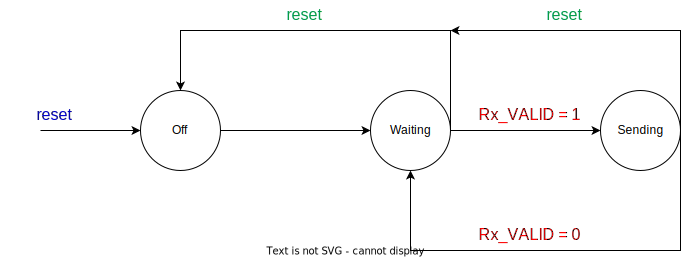
\includegraphics[width=\textwidth]{FSM.drawio.png} }
     	\caption{Moore FSM for connection}
     	\label{Moore FSM for connection}
     \end{figure}

    \section{\textcolor{PineGreen}{Testbench and Simulation}}
    Για το Simulation τροποποιήσαμε το Testbench του Reed-Solomon Decoder με σκοπό να προσομοιώσουμε την συνεχή ροή δεδομένων από ένα UART Transmitter προς τον UART Receiver του design μας. To Testbench ελέγχει 100 ακολουθίες αριθμών των 204 bytes η καθεμιά, τα οποία διαβάζει από ένα αρχείο και συγκρίνει τα αποτελέσματα του Decoder μέσω ενός άλλου αρχείου που περιέχει τα σωστά αποτελέσματα. Οπότε, το testbench κάνει αυτόματα τον έλεγχο και εάν βρεθεί κάποιο λάθος αναφέρει σε ποια γραμμή έγινε.\\
    Παράλληλα, μαζί με το design του decoder δόθηκε και ένα απλό script σε \verb|Matlab| όπου κάνει generate random περιπτώσεις 100 τέτοιων ακολουθιών και ταυτόχρονα παράγει και το αποτέλεσμα μετά την αποκωδικοποίηση. Οπότε μπορούν να δημιουργηθούν αμέτρητα tests για το συγκεκριμένο design. Εφόσον το input 204 bytes τα test που μπορουν να παραχθούν είναι άπειρα, οπότε για να επιβεβαιωθεί η σωστή λειτουργία του design θα έπρεπε να τεσταριστούν οριακές περιπτώσεις με βάση τον μαθηματικό αλγόριθμο που ακολουθεί το Reed Solomon. \\
    Παρακάτω φαίνονται κάποιες εικόνες από τις κυματομορφές του simulation, όπου στην πρώτη απεικονίζεται η μετάδοση των δεδομένων από τον Receiver στο Decoder. Ενώ, στην δεύτερη παρατηρούμε την διαδικασία αποκωδικοποίησης των δεδομένων από τον decoder.

    \begin{figure} [H]
     	\centering{\includegraphics[width=\textwidth]{Picture1.png} }
     	\caption{Data Transmission Waveforms}
     	\label{Data Transmission Waveforms}
     \end{figure}
     
    \begin{figure} [H]
     	\centering{\includegraphics[width=\textwidth]{Picture2.png} }
     	\caption{Decoded Data Output Waveforms}
     	\label{Decoded Data Output Waveforms}
     \end{figure}

     \section{\textcolor{PineGreen}{Real World Application}}
     Ο κώδικας Reed-Solomon χρησιμοποιείται συνήθως σε διάφορες εφαρμογές, όπως δορυφορικές επικοινωνίες και ψηφιακές συσκευές αποθήκευσης. Είναι ιδιαίτερα χρήσιμος σε περιπτώσεις όπου υπάρχει μεγάλη πιθανότητα εμφάνισης σφαλμάτων κατά τη μετάδοση ή την αποθήκευση δεδομένων, όπως σε θορυβώδη κανάλια επικοινωνίας ή σε περιβάλλοντα με υψηλές ηλεκτρομαγνητικές παρεμβολές.\\
     Οπότε το συγκεκριμένο design βρίσκει εφαρμογή σε όλες τις μεταφορές δεδομένων οι οποίες είναι ευάλωτες σε αλλοίωση των δεδομένων, δεδομένου ότι το transmission γίνεται με το πρωτόκολλο UART.

    \section{\textcolor{PineGreen}{Synthesis Process}}
    \subsection{\textcolor{PineGreen}{Top-Down view}}
    Για την διαδικασία της σύνθεσης χρειάστηκε να δημιουργήσουμε ένα script TCL συμβατό με τις εντολές του \verb|Genus| της \verb|Cadence|. Γενικότερα, η μέθοδος του top down στην σύνθεση είναι ότι παρέχεις στο εργαλείο όλα τα αρχεία της verilog και υλοποιεί την σύνθεση για όλο το κύκλωμα με βάση την ιεραρχεία.\newline
    Ξεκινήσαμε να δοκιμάζουμε για διάφορα ρολόγια σύνθεση, ξεκινώντας από τα 10ns έως τα 2ns όπου εκεί παραβιάζονταν το \textbf{slack} (δηλαδή μικρότερο του 50ps το οποίο είναι απαγορευτικό διότι θα προστεθούν και οι καθυστερήσεις των καλωδίων) οπότε ως optimal θεωρήθηκε το design με ρολόι 4ns περίοδο.\\
    Παρακάτω φαίνεται η καμπύλη pareto με την περίοδο σε σχέση με το area
    
   \begin{figure} [H]
    	\centering{\includegraphics[width=0.8\textwidth]{pareto.png} }
    	\caption{Pareto chart}
    	\label{pareto chart}
    \end{figure}

	\section{\textcolor{PineGreen}{Post-Synthesis Simulation}}
	Μετά την σύνθεση πήραμε το gate level design σε verilog και το sdf αρχείο που παράγει το genus με τις καθυστερήσεις της κάθε πύλης και έπρεπε να το προσωμοιώσουμε με το testbench, που είχαμε ήδη υλοποιημένο, στο Incisive.\\
	Εν τέλη, λόγω του όγκου του design η προσομοίωση του gate level στο Incisive ήταν αδύνατη, οπότε προσωμοιώσαμε το gate level στο Icarus χωρίς το sdf θεωρώντας πως οι καθυστερήσεις δεν θα επηρεάσουν την λειτουργία του. 
	
	??εικονα?? 
    
 	\section{\textcolor{PineGreen}{Placement Process}}
 	Για την διαδικασία του placement χρειάστηκε να υλοποιήσουμε ένα tcl script συμβατό με τις εντολές του \verb|Innovus| της \verb|Cadence|. Ξεκινήσαμε την διαδικασία του placement με τις default ρυθμίσεις που περιγράφονταν στο αντίστοιχο pdf. Ωστόσο, παρατηρήσαμε ότι στα timing reports είχαμε violations σε πολλά paths, κάποια από τα οποία δεν διορθώθηκαν μετά το optimisation.\\
 	Για να το διορθώσουμε αυξήσαμε το core utilization έως το 80\% και τα layers από 6 σε 7 αλλά δεν υπήρξε ουσιαστικό αποτέλεσμα. Τελικά, αλλάξαμε χειροκίνητα τα dimensions του design από $380 x 380$ σε $450 x 450$ και με τις υπόλοιπες ρυθμίσεις ως έχει και ενώ είχαμε αρνητικό slack μετά το optimisation το slack έγινε 0 ενώ επίσης και τα violating paths έγιναν 0 ενώ το density αυξήθηκε στο 61.18\%. Οπότε θεωρήσαμε ότι εφόσον δεν έχει violations είναι ιδανικό για να συνεχίσει η διαδικασία.\\
 	Στην συνέχεια δημιουργήσαμε το clock tree synthesis ορίζοντας τους buffers και τους inverters που χρειάζονται για το CTS και κάναμε και optimize το αποτέλεσμα. Ακολούθησε η υπόλοιπη διαδικασία που περιλαμβάνει το nano-routing και το optimize αυτού και λάβαμε τα τελικά reports που επιβεβαιώνουν την λειτουργικότητα του κυκλώματος και το power analysis το οποίο φαίνεται αναλυτικά στην εικόνα που ακολουθεί.
 	\begin{figure} [H]
 		\centering{\includegraphics[width=0.8\textwidth]{excel2.png} }
 		\caption{Power Results}
 		\label{Power Results}
 	\end{figure}
 
     Τέλος, ακολούθησε η διαδικασία του verification όπου ελέγχθηκε το geomtry και το connectivity όπου κανένα από τα δύο δεν εμφάνισε ούτε errors ούτε warnings.
     Ακολουθεί εικόνα από το placement όλων των cells και των καλωδίων όπως φαίνεται στο Innovus.\\
 	Παρακάτω φαίνονται τα συνολικά αποτελέσματα του placement πριν και μετά από το optimization
 	\begin{figure} [h]
 		\centering{\includegraphics[width=0.7\textwidth]{design with gates.png} }
 		\caption{Final Design}
 		\label{Final Design}
 	\end{figure}

    
 	
 	
\end{document}